\documentclass[tikz,border=6pt]{standalone}
\usepackage{tikz}
\usetikzlibrary{arrows.meta}
\definecolor{nebula}{HTML}{6366F1}
\definecolor{spark}{HTML}{14B8A6}
\definecolor{ink}{HTML}{334155}
\begin{document}
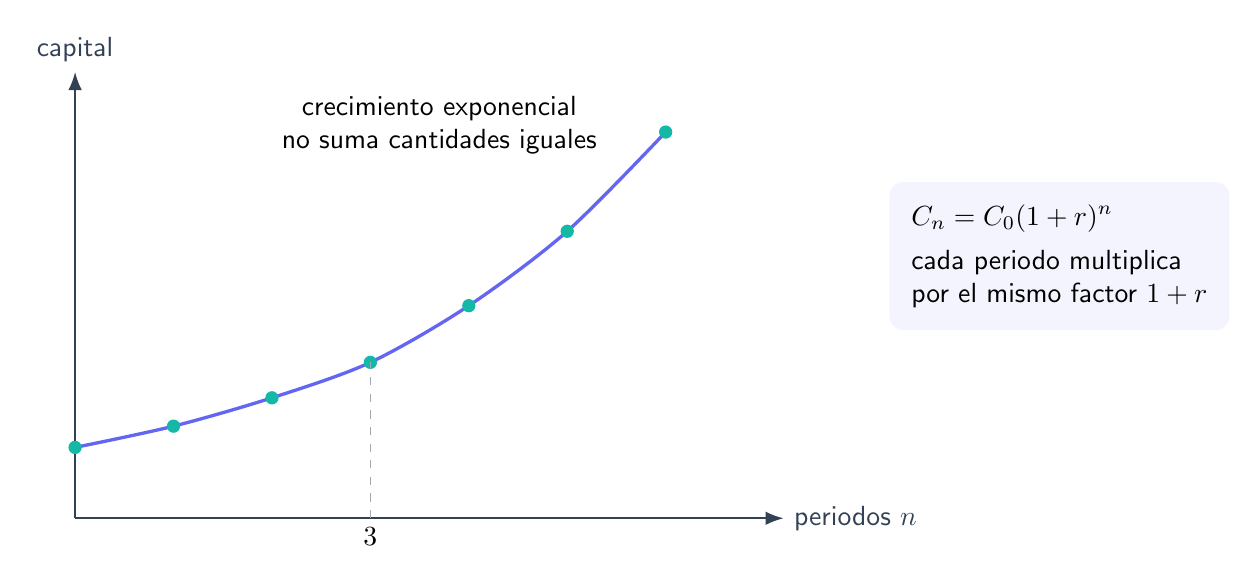
\begin{tikzpicture}[font=\sffamily,>=Latex,x=1.25cm,y=0.9cm]
  \draw[->,thick,ink] (0,0)--(7.2,0) node[right] {periodos $n$};
  \draw[->,thick,ink] (0,0)--(0,6.3) node[above] {capital};
  \draw[very thick,nebula] plot[smooth] coordinates {(0,1)(1,1.3)(2,1.7)(3,2.2)(4,3)(5,4.05)(6,5.45)};
  \foreach \x/\y in {0/1,1/1.3,2/1.7,3/2.2,4/3,5/4.05,6/5.45}{\fill[spark] (\x,\y) circle(2.4pt);}
  \draw[dashed,ink!45] (3,0)--(3,2.2);
  \node[below] at (3,0) {$3$};
  \node[align=left,fill=nebula!7,rounded corners=5pt,inner sep=8pt] at (10,3.7) {$C_n=C_0(1+r)^n$\\[4pt]cada periodo multiplica\\por el mismo factor $1+r$};
  \node[align=center,fill=white] at (3.7,5.55) {crecimiento exponencial\\no suma cantidades iguales};
\end{tikzpicture}
\end{document}
